\documentclass{article}

\usepackage[backend=biber]{biblatex}
\addbibresource{metabolic.bib}

\usepackage{amsmath,amsfonts}

\usepackage{tikz}
\usetikzlibrary{positioning,matrix}

\title{Learning an integrated network of metabolites, lipids, and proteins from knockout screens}

\author{Yuriy Sverchkov}

\begin{document}
\maketitle

\begin{abstract}
Learning an integrated network of metabolites and proteins from knockout (KO) screens.
Given knockout screens with large-scale MS measurements of protein, metabolite, and lipid abundances, as well as incomplete prior knowledge about
relevant regulatory, signaling, and metabolic pathways, we seek to elucidate the roles of uncharacterized actors and extend the network accordingly.
\end{abstract}

\section{Introduction}

%TODO State clearly our goals

\section{Background}

Prior related work includes:
\begin{itemize}
 \item \textcite{lee2008dynamic} present a flux-balance-analysis-based model that integrates signaling, metabolic, and regulatory networks.
\end{itemize}

Our approach is in some ways similar to nested effects model \parencite{citation-needed}.
A general effects model can be characterized by an effect matrix $F$ where columns correspond to knockouts and and the rows correspond to measured phenotypes or ``effects,'' and matrix entries correspond to differential expression.
The NEM factorizes $F = \Gamma \Theta$ where $\Gamma$ represents the propagation of a knockout to changes in gene activity among signaling genes (assumed to be the set of genes knocked out) and $\Theta$ represents the propagation of those changes to the measured effects.

\section{General approach}

The task at hand is that of refining and (in some aspects) de-novo constructing a network of interactions between genes, proteins, metabolites, and lipids.
We approach the problem as one of synthesizing data and prior knowledge, more concretely:

\begin{itemize}
 \item \emph{The data} consists of log fold change for KO relative to wild type particle abundance measurements, derived from mass spectrometry (MS).
 \begin{itemize}
  \item Proteomics
  \item Metabolomics
  \item Lipidomics
 \end{itemize}
 \item \emph{The prior knowledge} comes in the form of networks of interactions available from a variety of sources.
 \begin{itemize}
  \item Gene and protein interaction networks
  \item Metabolic networks: KEGG, BioCyc.
  \item There are no networks for lipids.
 \end{itemize}
\end{itemize}

See Section~\ref{sec:data} for more about our data.
We attempt to integrate this data and prior knowledge into \emph{a model that explains how the changes introduced by a KO propagate to the measurements}.
Figure~\ref{fig:high-level} is a high-level diagram of this propagation.

\begin{figure}
\centering
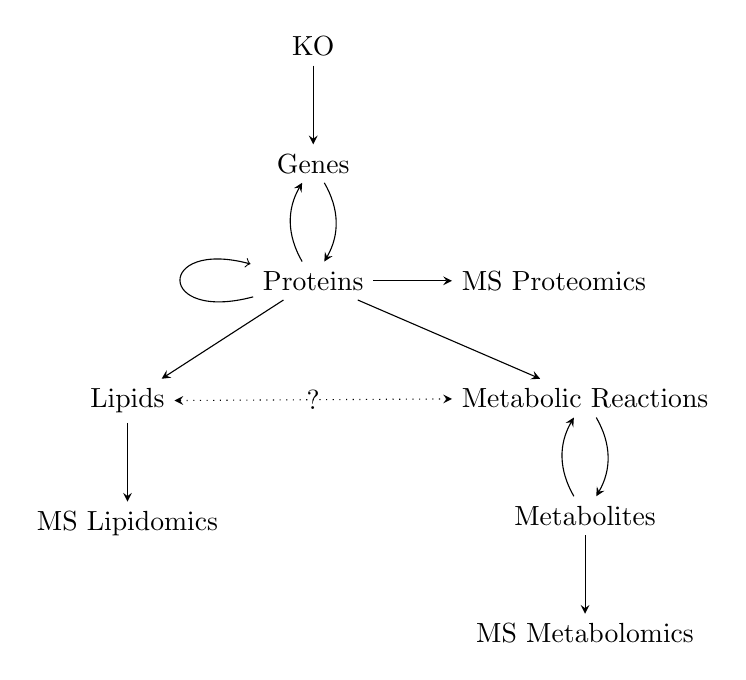
\begin{tikzpicture}
  \node (ko) {KO};
  \node (genes) [below=of ko] {Genes};
  \node (proteins) [below=of genes] {Proteins};
  \node (proteomics) [right=of proteins] {MS Proteomics};
  \node (reactions) [below right=of proteins] {Metabolic Reactions};
  \node (metabolites) [below=of reactions] {Metabolites};
  \node (metabolomics) [below=of metabolites] {MS Metabolomics};
  \node (lipids) [below left=of proteins] {Lipids};
  \node (lipidomics) [below=of lipids] {MS Lipidomics};
  
  \path[-stealth]
    (ko) edge (genes)
    (genes) edge [bend left] (proteins)
    (proteins) edge [bend left] (genes)
    (proteins) edge [loop left] (proteins)
    (proteins) edge (proteomics)
    (proteins) edge (reactions)
    (reactions) edge [bend left] (metabolites)
    (metabolites) edge [bend left] (reactions)
    (metabolites) edge (metabolomics)
    (proteins) edge (lipids)
    (lipids) edge (lipidomics)
    (lipids) edge [stealth-stealth,dotted] node {?} (reactions);

\end{tikzpicture}
\caption{A high-level diagram of how the changes introduced by a KO propagate to the measurements.}
\label{fig:high-level}
\end{figure}

\paragraph{Observation.}
If we can assume that there is no pathway for KOs to affect metabolites other than via its effect on proteins, we could treat the problem of predicting changes in metabolites given changes in proteins as a distinct problem from that of predicting changes in proteins KOs.
The main issue with this approach is that our measurements of proteins in some cases identifies protein groups (since protein identification is based on peptides).

\section{Naive model statement}

We can simplify some of the complexity of Figure~\ref{fig:high-level} by collapsing gene-protein, protein-protein, and gene-gene interactions into a single model through identification of genes with the proteins they code for, yielding a simplified model shown in Figure~\ref{fig:simplified-proteins}.

\begin{figure}
\centering
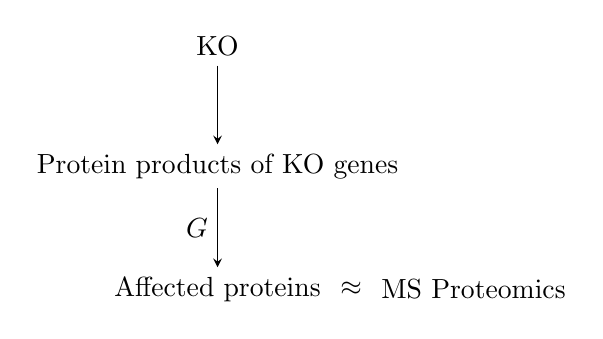
\begin{tikzpicture}
  \node (ko) {KO};
  \node (target) [below=of ko] {Protein products of KO genes};
  \node (proteins) [below=of target] {Affected proteins};
  \node (eqsign) [anchor=west] at (proteins.east) {$\approx$};
  \node (proteomics) [anchor=west] at (eqsign.east) {MS Proteomics};
  
  \path[-stealth]
    (ko) edge (target)
    (target) edge node [left] {$G$} (proteins);
\end{tikzpicture}
\caption{A simplified model for propagation of knockouts to proteins.}
\label{fig:simplified-proteins}
\end{figure}

\paragraph{Knockout-protein model.}
The matrix $G$ models how proteins interact, more specifically, how the abundance of one protein affects the abundance of another.
This means that entities like protein complexes are only relevant in interactions if they in turn affect the abundances of other proteins (e.g. by affecting regulation).
If we suppose that there is a graph that represents protein interactions, and suppose that in the experiment, there is sufficient time for the effects of knockouts to propagate throughout the graph, $G$ is the transitive closure of the graph.
Moreover, if a change is observed in one protein, the effects of that change must have been observed as well in all proteins affected by that protein.
If we had access to the true effect matrix $F$, we would have:
\begin{itemize}
 \item $F_{i \cdot} S = F_{i \cdot}$ for each knockout $i$. This is because if a change is observed in a protein, the propagation of that change to other proteins must have also been observed.
 \item If $F_{i j} = F_{i' j} \neq 0$ then $\forall k : S_{j k} \neq 0 \Rightarrow F_{i k} = F_{i' k}$.
 \item $S_{i \cdot} = F_{i \cdot}$.
\end{itemize}
Note that the statements above are not orthogonal.

\paragraph{Protein-metabolite model.}
To easily incorporate known metabolic pathways into the model we first start with the formulation of a pair of binary matrices, $R^\text{in}$ and $R^\text{out}$, where each row corresponds to a reaction and each column a metabolite.
$R^\text{in} - R^\text{out}$ is somewhat similar to a flux matrix, but we don't model stoichiometry here.\footnote{Could we model stoichiometry?}
We also need a matrix that tells us which protein catalyzes which reaction.
Let that be a binary matrix $C$, where each row is a protein and each column is a reaction.
Given these, $C R^\text{in}$ and $C R^\text{out}$ give us matrices where each row is a protein, and each column is a metabolite that potentially accumulates/depletes due to a change in the protein-catalyzed reactions associated.
These changes may in turn propagate through the metabolic network.
To model this propagation we can consider, for a given protein presence/absence vector $\vec p$, $(R^\text{in})^T ( \vec p C ) R^\text{out}$ as the propagation model.
Therefore, given protein presence/absences vector $\vec p$ and protein abundance change vector $\vec{\Delta p}$, the expected change in the metabolite vector $\vec{ \Delta m}$ is bounded as:\footnote{We use $\cdot^\infty$ to represent transitive closure. We could also potentially use something like a diffusion model instead of a proper closure.}
\[
 -\vec{\Delta p} C R^\text{out} ( (R^\text{in})^T ( \vec p C ) R^\text{out} )^\infty \leq \vec{ \Delta m} \leq \vec{\Delta p} C R^\text{in} ( (R^\text{in})^T ( \vec p C ) R^\text{out} )^\infty
\]
One implicit assumption is that changes in abundance don't propagate backwards: the accumulation of a product of a reaction does not get potentially propagated to accumulations of the ingredients.

A relaxed version of this model is one that does not take into account the change in available reactions in propagation, this simplifies to
\begin{equation} \label{eq:metabolite-bounds}
 -\vec{\Delta p} C R^\text{out} \underbrace{( (R^\text{in})^T R^\text{out} )^\infty}_M \leq \vec{ \Delta m} \leq \vec{\Delta p} C R^\text{in} \underbrace{( (R^\text{in})^T R^\text{out} )^\infty}_M
\end{equation}
where M is the transitive closure of the metabolic network (for metabolites).

\subsection{Statement as a likelihood}

\paragraph{The protein model.}
The protein model consists of a single, transitively closed, trinary $(-1, 0, 1)$ matrix $G$, but for the optimization formulation, it helps to separate it into two matrices, making up the positive and negative components, $G_+$ and $G_-$ respectively.
We then have the constraints:
\begin{align}
 \left. \begin{aligned}
  G_{+ij} \in \{0,1\} \\
  G_{-ij} \in \{0,1\}
 \end{aligned} \right\} \forall i,j
 &\qquad \text{Domain constraints} \\
 G_{+ij} + G_{-ij} \leq 1 \quad \forall i,j &\qquad \text{Logical consistency constraint} \\
 \left. \begin{aligned}
  G_{+ij} \geq G_{+ik} G_{+kj} \\
  G_{+ij} \geq G_{-ik} G_{-kj} \\
  G_{-ij} \geq G_{-ik} G_{+kj} \\
  G_{-ij} \geq G_{+ik} G_{-kj}
 \end{aligned} \right\} \forall i,j,k
 &\qquad \text{Transitivity constraints}
\end{align}

To derive the likelihood, we view this as a generative model where
\begin{equation}
 D_{ij} = f( G_{ij} )
\end{equation}
For Knockut $i$ and protein $j$, where $f$ is a function from the $\{ -1, 0, 1\}$ space to the space of $D$.
The likelihood part of the optimization is then simply $\sum_{ij} \ell ( i j )$ for pointwise likelihood function $i j$.

\paragraph{Optimizing transitivity.}
The transitive constraints in the na\:ive formulation are quadratic, however, we can replace $G_+, G_-$ with a variable $T$ representing all three-node-paths, defining
\begin{align}
 T_{i+j+k} = G_{+ij} G_{+jk} \quad; i \rightarrow^+ j \rightarrow^+ k \\
 T_{i+j-k} = G_{+ij} G_{-jk} \quad; i \rightarrow^+ j \rightarrow^- k \\
 T_{i-j+k} = G_{-ij} G_{+jk} \quad; i \rightarrow^- j \rightarrow^+ k \\
 T_{i-j-k} = G_{-ij} G_{-jk} \quad; i \rightarrow^- j \rightarrow^- k
\end{align}
where some of these paths are predefined/identical by definition:
\begin{alignat}{3}
 T_{i+i+i} = 1 \qquad & T_{i-i \cdot \cdot} = 0 \qquad & T_{ \cdot \cdot i - i } = 0 \\
 T_{i+i \cdot j} = T_{i \cdot j+j} \qquad &
\end{alignat}
and, as a result, we can represent the transitivity constraints as linear.
However, we need to introduce a constraint for $T$ to accurately maintain its meaning, namely, $T_{i+j+k} = T_{i+j+j} T_{j+j+k}$, which can be rewritten as
\begin{gather}
  T_{i x j \cdot k} \leq T_{i x j+j} \qquad T_{i \cdot j x k} \leq T_{j x k + k} \\
  T_{i x j y k} \geq T_{i x j + j} + T_{j y k + k} - 1
\end{gather}
with $i,j,k$ in the protein space and $x,y \in \{+,-\}$.

$T$ is therefore a tensor in $\mathbb R^{n \times 2 \times n \times 2 \times n}$ if we are given $n$ proteins.
By careful parametrization we can eliminate redundant model parameters, but the number of parameters and constraints is unavoidably going to be on the order of $n^3$ when formulated as a linear problem.

\paragraph{The metabolite and lipid model.}
The objective function is constructed as a function that penalizes the violations of the bounds in Equation~\eqref{eq:metabolite-bounds}.
The optimization for the metabolite model similarly requires a set of transitivity constraints.

\section{Towards a simplified propagation model}

\begin{itemize}
 \item A transitively closed ``detailed'' graph captures the model of propagation of the perturbation by the knockout to measurable effects, the number of nodes in such a graph is at least on the order of the sum of knockouts and effects.
 \item A transitively closed graph can be factored into a tri-partite graph of knockouts to latent components to effects.
 \item The NEM model places a constraint on the number and nature of the latent components.
 \item The NEM model constraints are such that there exist transitively closed detailed graphs that are not expressible by an NEM, leading one to either (1) relax the constraint on latent components or (2) relax the constraint on effect associations.
 \item My aim is to come up with a model formulation that is (1) tri-partite (2) significantly more compact than the detailed transitively closed graph and (3) as expressive as the transitively closed graph when it comes to propagation of changes from KOs to effects.
 \item The tri-partite representation bears similarity to topic models, can those methods be adapted for this setting?
\end{itemize}

\subsection{Connection to NEMs}

Some of the statements above may not be obvious, the first being the view of an NEM as a tri-partite graph, after all, an NEM is usually presented as a (often transitively closed) graph over the KO genes and one-way connections to effects.
Figure~\ref{fig:nem-tri} illustrates how we can view an NEM model as a tri-partite one-directional graph of KOs to gene sets to effects, and in fact, that view corresponds directly to the matrix decomposition of the model.

\begin{figure}
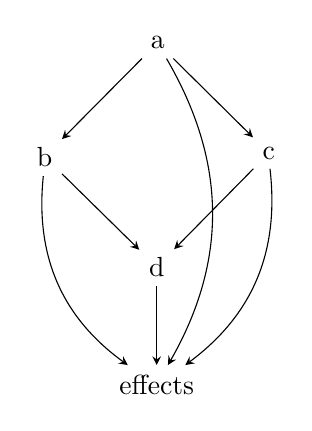
\begin{tikzpicture}

  \node (a) {a};
  \node (b) [below left=of a] {b};
  \node (c) [below right=of a] {c};
  \node (d) [below left=of c] {d};
  \node (ef) [below=of d] {effects};
  
  \path[-stealth]
    (a) edge (b)
    (a) edge (c)
    (b) edge (d)
    (c) edge (d)
    (a) edge [bend left] (ef)
    (b) edge [bend right] (ef)
    (c) edge [bend left] (ef)
    (d) edge (ef);

\end{tikzpicture}
%
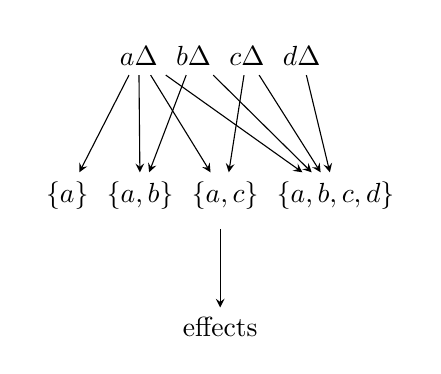
\begin{tikzpicture}
  \matrix (ko) [matrix of math nodes]
  { a \Delta & b \Delta & c \Delta & d \Delta \\ };
  \matrix (set) [matrix of math nodes, below=of ko]
  { \{ a \} & \{ a, b \} & \{ a, c \} & \{ a, b, c, d \} \\ };
  \node (effects) [below=of set] {effects};
  
  \path[-stealth]
    (ko-1-1) edge (set-1-1)
    (ko-1-1) edge (set-1-2)
    (ko-1-1) edge (set-1-3)
    (ko-1-1) edge (set-1-4)
    (ko-1-2) edge (set-1-2)
    (ko-1-2) edge (set-1-4)
    (ko-1-3) edge (set-1-3)
    (ko-1-3) edge (set-1-4)
    (ko-1-4) edge (set-1-4)
    (set) edge (effects);

\end{tikzpicture}

\caption{Illustration of the classical graphic representation of an NEM and a tri-partite representation.}
\label{fig:nem-tri}
\end{figure}

What the classical NEM model does with respect to the latent layer is place strict constraints on the size (equal to the number of KO genes), interpretation (Each is associated primarily with a KO gene), and relationships between the latent variables.\footnote{I'd like two write out explicitly what these constraints on relationships are, but it is not so simple. Something along the lines of ``for each KO gene $g$ there must exist a set $S_g$ in which it appears such that if the gene $g$ appears in any other set $S_x$, then $S_q \subset S_x$.'' I have yet to verify wether this is a complete characterization of the constraint.}

\subsection{Naive representation of a transitive graph as tri-partite and reduction}

Suppose (as in our problem) we have proteins $a,b,c,d$ governed by some causal graph (Figure~\ref{fig:general-tri}) where we only have KO's of two proteins that correspond to genes, $a\Delta$ and $b\Delta$, and we have measurements of all proteins (as in our problem).
The accessibility matrix of the graph is

\begin{figure}
\begin{tikzpicture}
  \node (a) {a};
  \node (c) [below right=of a] {c};
  \node (b) [above right=of c] {b};
  \node (d) [below right=of b] {d};
  \node (ako) [above=of a] {$a\Delta$};
  \node (bko) [above=of b] {$b\Delta$};
  
  \path[-stealth]
    (ako) edge (a)
    (bko) edge (b)
    (a) edge (c)
    (b)
      edge (c)
      edge (d);
\end{tikzpicture}
%
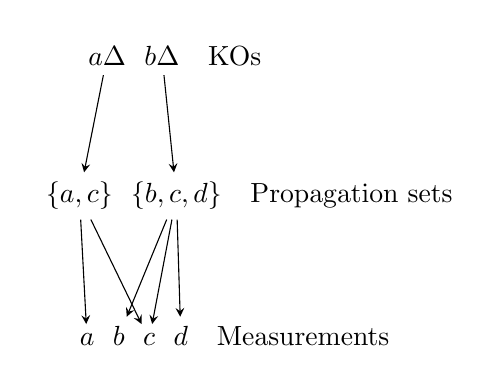
\begin{tikzpicture}
  \matrix (ko) [matrix of math nodes]
  { a \Delta & b \Delta \\ };
  \matrix (set) [matrix of math nodes, below=of ko]
  { \{ a, c \} & \{ b, c, d \} \\ };
  \matrix (ef) [matrix of math nodes, below=of set]
  { a & b & c & d \\ };
  \node [anchor=west] at (ko.east) {KOs};
  \node [anchor=west] at (set.east) {Propagation sets};
  \node [anchor=west] at (ef.east) {Measurements};
  
  \path[-stealth]
    (ko-1-1) edge (set-1-1)
    (ko-1-2) edge (set-1-2)
    (set-1-1)
      edge (ef-1-1)
      edge (ef-1-3)
    (set-1-2)
      edge (ef-1-2)
      edge (ef-1-3)
      edge (ef-1-4);
  
\end{tikzpicture}
%
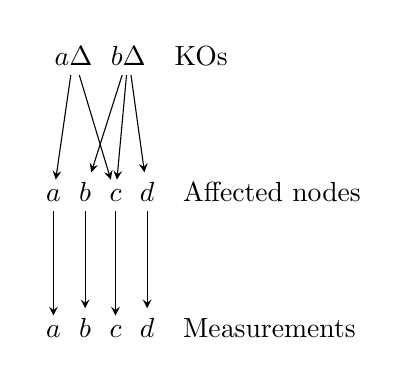
\begin{tikzpicture}
  \matrix (ko) [matrix of math nodes]
  { a \Delta & b \Delta \\ };
  \matrix (set) [matrix of math nodes, below=of ko]
  { a & b & c & d \\ };
  \matrix (ef) [matrix of math nodes, below=of set]
  { a & b & c & d \\ };
  \node [anchor=west] at (ko.east) {KOs};
  \node [anchor=west] at (set.east) {Affected nodes};
  \node [anchor=west] at (ef.east) {Measurements};
  
  \path[-stealth]
    (ko-1-1)
      edge (set-1-1)
      edge (set-1-3)
    (ko-1-2)
      edge (set-1-2)
      edge (set-1-3)
      edge (set-1-4)
    (set-1-1) edge (ef-1-1)
    (set-1-2) edge (ef-1-2)
    (set-1-3) edge (ef-1-3)
    (set-1-4) edge (ef-1-4);
  
\end{tikzpicture}
%
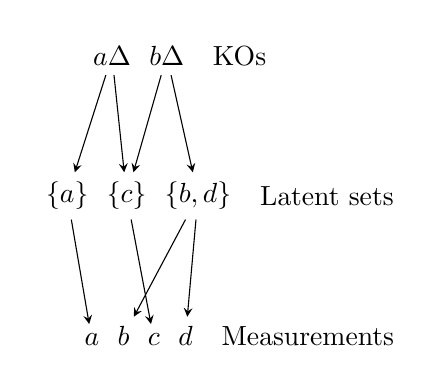
\begin{tikzpicture}
  \matrix (ko) [matrix of math nodes]
  { a \Delta & b \Delta \\ };
  \matrix (set) [matrix of math nodes, below=of ko]
  { \{a\} & \{c\} & \{b,d\} \\ };
  \matrix (ef) [matrix of math nodes, below=of set]
  { a & b & c & d \\ };
  \node [anchor=west] at (ko.east) {KOs};
  \node [anchor=west] at (set.east) {Latent sets};
  \node [anchor=west] at (ef.east) {Measurements};
  
  \path[-stealth]
    (ko-1-1)
      edge (set-1-1)
      edge (set-1-2)
    (ko-1-2)
      edge (set-1-2)
      edge (set-1-3)
    (set-1-1) edge (ef-1-1)
    (set-1-2) edge (ef-1-3)
    (set-1-3)
      edge (ef-1-2)
      edge (ef-1-4);
  
\end{tikzpicture}
\caption{Illustration of possible mappings of a transitive graph to a tri-partite graph.}
\label{fig:general-tri}
\end{figure}

\begin{equation}
  G =
  \begin{pmatrix}
   1 & 0 & 1 & 0 \\
   0 & 1 & 1 & 1 \\
   0 & 0 & 1 & 0 \\
   0 & 0 & 0 & 1
  \end{pmatrix}
\end{equation}
of which we only observe two rows that correspond to the performed KOs, namely
\begin{equation}
  F =
  \begin{pmatrix}
   1 & 0 & 1 & 0 \\
   0 & 1 & 1 & 1 \\
  \end{pmatrix}
  \text{.}
\end{equation}

Intuitively, one can consider making the latent layer correspond to either the sets of nodes affected by a KO or the nodes affected by a KO, but those two extremes correspond to trivial factorizations where either the KO $\rightarrow$ latent layer or latent layer $\rightarrow$ KO connections fully capture $G$.
A more informative model that I propose borrows from NEMs, but is slightly less restrictive: each measurement connects to at most one latent node, and no pair of latent nodes connect to the same set of KO's.
In such a representation, because each measurement is assigned to at most one latent node, the latent nodes implicitly represents sets of elements (proteins in our protein sub-problem).
Once we have the sets, a DAG based on subset relations among them can be reconstructed.
Such a DAG would be similarly interpreted to an NEM, representing causal relationships.

\paragraph{Learning latent sets in the ideal case.}
In the ideal case, the latent sets correspond to unique columns of $F$, they can be read off from the data.

\section{Data}

The data we have is $\log_2$-fold change in KO vs WT data.
As of April 2nd, 2018, we have the following data:


%%%\section{Results}

%%%\section{Discussion}

\printbibliography

\end{document}